\chapter{Volatility Modelling}
In this chapter, we will...
\section{(Rough) Stochastic Volatility Models}
The motivation for the development of stochastic volatility models was the constant volatility assumption of the Black \& Scholes model, which proved to be incompatible with observed market option prices. Hence, stochastic volatility models must also specify the stochastics of the volatility process. One of the most popular stochastic volatility models is the Heston model, which is specified by the pair of SDEs
\begin{align}
    dS_{t}&= \mu S_{t}dt + \sqrt{\nu_{t}}S_{t}dB_{t}^{(1)},\\
    d\nu_{t}&= \kappa(\theta - \nu_{t})dt + \xi\sqrt{\nu_{t}}dB_{t}^{(2)},
\end{align}
where $\langle B^{(1)},B^{(2)}\rangle_{t}=\rho t$ with $|\rho|\leq 1$. The first SDE specifies the dynamics for the underlying asset $S_{t}$, and the second SDE is a Cox-Ingersoll-Ross process specifying the dynamics of the variance process $\nu_{t}$. Additionally, it is assumed that $S_{0},\nu_{0}>0$, and that the so-called Feller condition $2\kappa\theta >\xi^{2}$ is satisfied ensuring the variance process is strictly positive. The parameter $\theta>0$ is the long-run variance, $\kappa$ governs the speed of reversion of $\nu_{t}$ towards $\theta$, and $\xi$ is the variance of $\nu_{t}$.

For a given set of model parameters, we can simulate the paths of $S_{t}$ and $\nu_{t}$ on $[0,T]$ by the following Euler-Maruyama scheme
\begin{align}
    \nu_{t_{k}}^{N}&= \nu_{t_{k-1}}^{N} + \kappa(\theta-\nu_{t_{k-1}}^{N})\Delta_{N} + \xi\sqrt{\nu_{t_{k-1}}^{N}}\sqrt{t_{k}-t_{t_{k-1}}}\zeta_{k}^{(1)}, \quad \nu_{0}^{N}=\nu_{0},\\
    S_{t_{k}}^{N}&= S_{t_{k-1}}^{N} + \mu S_{t_{k-1}}^{N}\Delta_{N} + \sqrt{\nu_{t_{k-1}}^{N}}S_{t_{k-1}}^{N}\sqrt{t_{k}-t_{t_{k-1}}}\zeta_{k}^{(2)}, \quad S_{0}^{N}=S_{0},
\end{align}
for $N\in\N$, $\Delta_{N}=T/N$, and $k=1,\dots,N$. Furthermore
\begin{equation}
    \begin{pmatrix}
        \zeta_{k}^{(1)}\\
        \zeta_{k}^{(2)}
    \end{pmatrix} \sim \mathcal{N}(0,\Sigma),\quad \Sigma = \begin{pmatrix}
        1 & \rho \\
        \rho & 1
    \end{pmatrix}.
\end{equation}
The Heston model will serve as a comparative model for our rough volatility model.
\subsection{Fractional Ornstein-Uhlenbeck Process}
The rough volatility model (rVol) that we will consider, models the volatility process via the fractional Ornstein-Uhlenbeck process
\begin{align}
    dY_{t}&= -\lambda(Y_{t}-\theta)dt + \varphi dB^{H}_{t}\\
    \sigma_{t} &= e^{Y_{t}},
\end{align}
where $\theta\in \R$, $\lambda,\varphi >0$, and $B^{H}$ is a fBM of Hurst index $H\in(0,1/2)$. As for the usual Ornstein-Uhlenbeck process, there is an explicit form for the solution
\begin{equation}\label{ornstein_sol}
    Y_{t}= \theta + (Y_{0}-\theta)e^{-\lambda t} + \varphi e^{-\lambda t}\int_{0}^{t}e^{\lambda s}dB_{s}^{H}.
\end{equation}
The integral in \eqref{ornstein_sol} can in accordance with Proposition \ref{thm:integration} be calculated as the pathwise Riemann-Stieltjes integral
\begin{equation}\label{eq:riemann}
    \int_{0}^{t}e^{\lambda s}dB_{s}^{H}=\lim_{N\to\infty}\sum_{k=0}^{N-1}e^{\lambda k t/N}\left(B_{(k+1)t/N}^{H}-B_{kt/N}^{H}\right).
\end{equation}
Thus, for $N\in\N$ sufficiently large, the above Riemann-sum will approximate the integral in \eqref{ornstein_sol} well. Changing the summation index in \eqref{eq:riemann}, we introduce the quantity
\begin{equation}
    \mathbb{B}_{t}^{H,N}\coloneqq \sum_{l=1}^{\lfloor Nt\rfloor }e^{\lambda l/N}\left(B^{H}_{l/N}-B^{H}_{(l-1)/N}\right)
\end{equation}
Thus, we can simulate a fractional Ornstein-Uhlenbeck process on the grid $0=t_{0}<t_{1}<\dots<t_{N}=T$ by the following 
\begin{equation}\label{fou_exact}
    Y_{t_{j}}^{N}=\theta + (Y_{0}-\theta)e^{-\lambda t_{j}} + \varphi e^{-\lambda t_{j}}\mathbb{B}_{t_{j}}^{H,N},\quad Y_{0}^{N}=Y_{0}, \quad j=1,\dots,N.
\end{equation}
Alternatively, we could use the Euler-Maruyama scheme to simulate the process
\begin{equation}\label{fou_euler}
    Y_{t_{j}}^{N}=Y_{t_{j-1}} -\lambda(Y_{t_{j-1}}-\theta)\Delta_{N} + \varphi\Delta B_{t_{j-1}}^{H},\quad Y_{0}^{N}=Y_{0},\quad j=1,\dots,N.
\end{equation}
The error rates for the two simulation methods in \eqref{fou_exact} and \eqref{fou_euler} are approximately the same, and since the Euler-Maruyama scheme is computationally faster, we will use the methodology in \eqref{fou_euler} for simulation. If we take the model 
\begin{equation}
    dY_{t}=-(Y_{t}-1)dt+\frac{1}{2}dB^{0.2}_{t},\quad Y_{0}=0,
\end{equation}
and use \eqref{fou_exact} with $N=100,000$ as our true solution path $Y_{t}$, then we can compare the Euler-approximations below.
\begin{figure}[H]
    \centering
    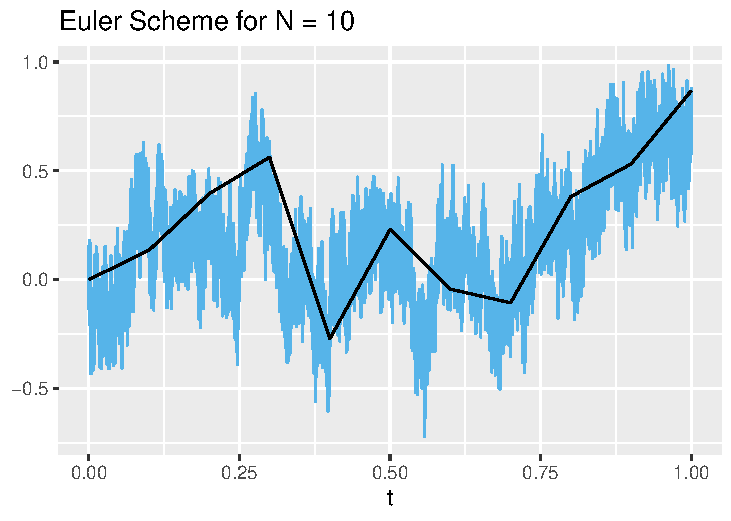
\includegraphics[scale=0.58]{fig/img/EulerScheme/EulerScheme10.pdf}\hfill
    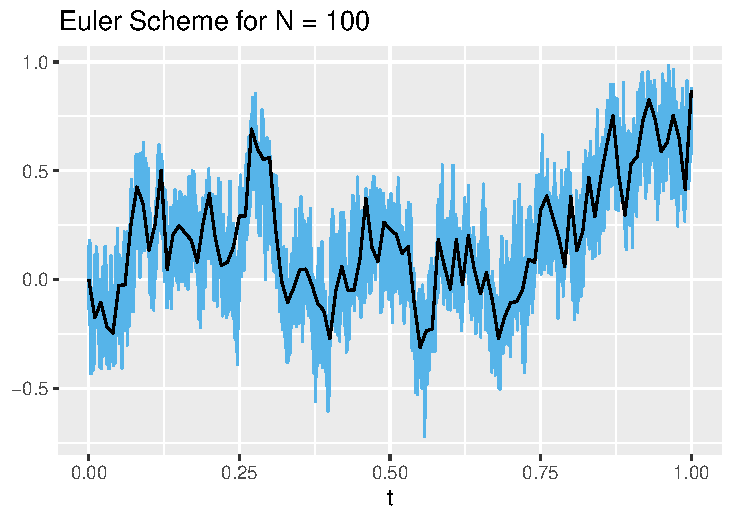
\includegraphics[scale=0.58]{fig/img/EulerScheme/EulerScheme100.pdf}\hfill
    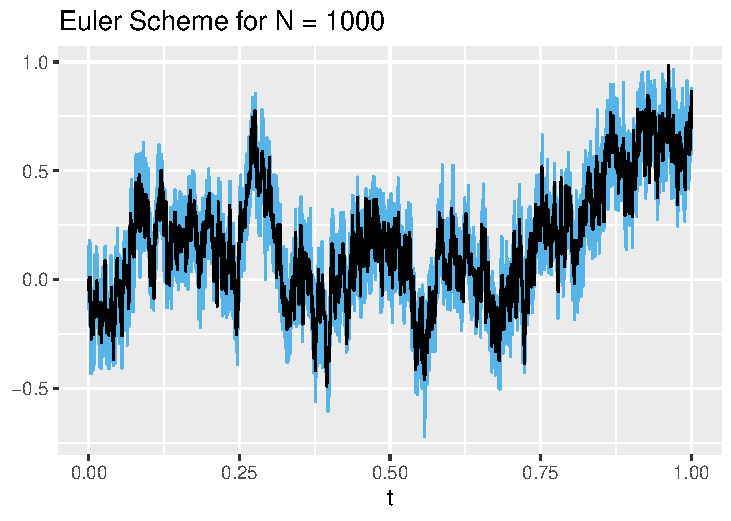
\includegraphics[scale=0.58]{fig/img/EulerScheme/EulerScheme1000.pdf}
    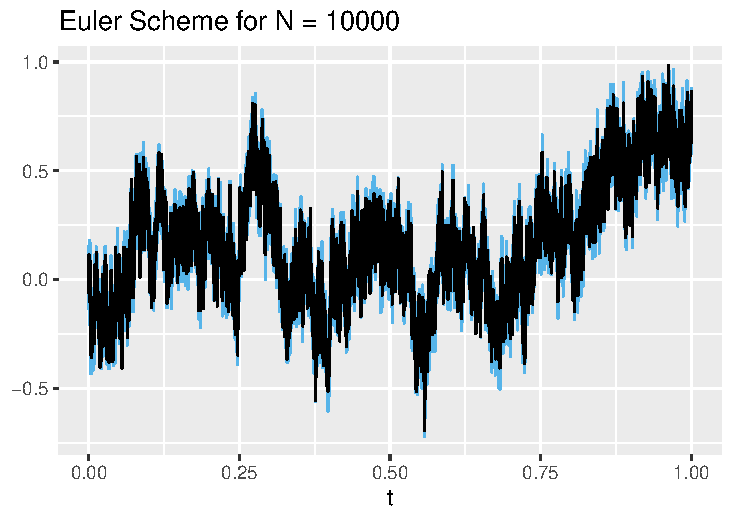
\includegraphics[scale=0.58]{fig/img/EulerScheme/EulerScheme10000.pdf}
    \caption{Euler Approximations for Various Step Sizes $\Delta_{N}$. }
    \label{fig:enter-label}
\end{figure}

\section{Volatility is Rough}
This section is based on \cite{volisrough}.

In this section, we will use the methodology presented in \cite{volisrough} to estimate the roughness of the volatility process. Suppose we have discrete observations of the volatility process $\sigma$ on the interval $[0,T]$ with mesh size $\Delta$, i.e. $\sigma_{0},\sigma_{\Delta},\dots,\sigma_{N\Delta}$ with $N\coloneqq \lfloor T/\Delta\rfloor$. Then for $q\geq 0$, we define the statistic
\begin{equation}
    m(q,\Delta)\coloneqq \frac{1}{N}\sum_{k=1}^{N}|\log(\sigma_{k\Delta})-\log(\sigma_{(k-1)\Delta})|^{q}.
\end{equation}
It is assumed that for some $s_{q}>0$ and $b_{q}>0$, we have
\begin{equation}\label{weirdlim}
    N^{qs_{q}}m(q,\Delta)\to b_{q}\quad \textrm{as}\quad \Delta\to 0^{+}.
\end{equation}
Under additional technical conditions, $s_{q}$ can be viewed as the regularity of the volatility. In particular, a function satisfying \eqref{weirdlim} is Hölder continuous with Hölder exponent $\alpha$ for any $\alpha <s_{q}$. For instance, if $\log(\sigma_{t})$ was a fBM with Hurst index $H$, then \eqref{weirdlim} would hold in probability with $s_{q}=H$ for any $q\geq 0$.

To estimate the smoothness parameter $s_{q}$ for each $q$, we compute $m(q,\Delta)$ for different $\Delta$ and regress $\log(m(q,\Delta))$ against $\log(\Delta)$. Since the volatility process is not directly observable, we have to proxy the true spot volatility. For this purpose, we use the daily realized variance estimates of the Oxford-Man Institute of Quantitative Finance Realized Library as our proxy for daily spot variance. The daily realized variance is calculated using intradaily intervals of 5 minutes over the 8 hour trading day of the S\&P-500 index. The data starts at 1/3-2000 and ends at 3/31-2020 totalling 5079 trading days. A plot of the data is seen in Figure \ref{fig:realized} along with the realized volatility (square root of the data).

\begin{figure}[H]
    \centering
    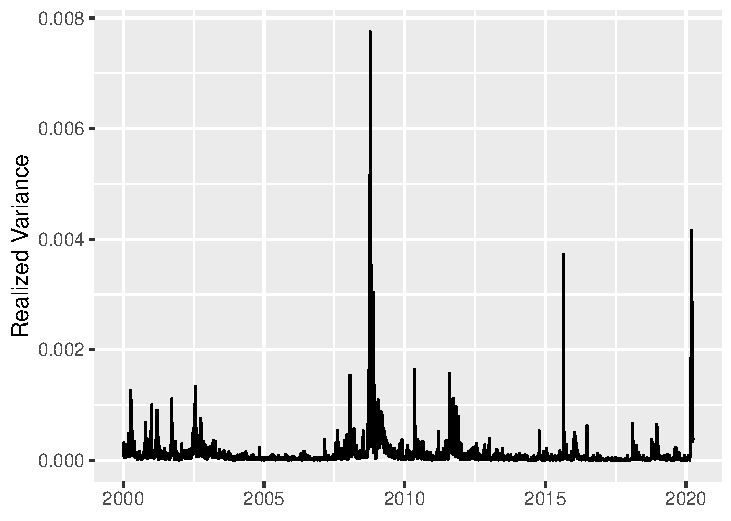
\includegraphics[scale=0.6]{fig/img/RealizedLib/SP500Realized.pdf}
    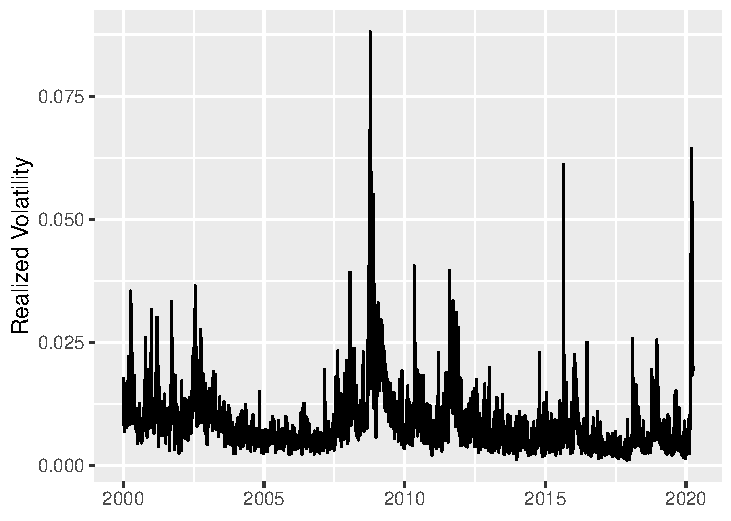
\includegraphics[scale=0.6]{fig/img/RealizedLib/SP500RealizedVol.pdf}
    \caption{Realized Variance (left) and Volatility (right) of the S\&P-500.}
    \label{fig:realized}
\end{figure}
We proceed to compute $m(q,\Delta)$ for $q\in \{0.5,1,1.5,2,3\}$ and $\Delta \in \{1,2,\dots,30\}$, and regress $\log(m(q,\Delta))$ against $\log(\Delta)$. As seen in Figure 
\begin{figure}[H]
    \centering
    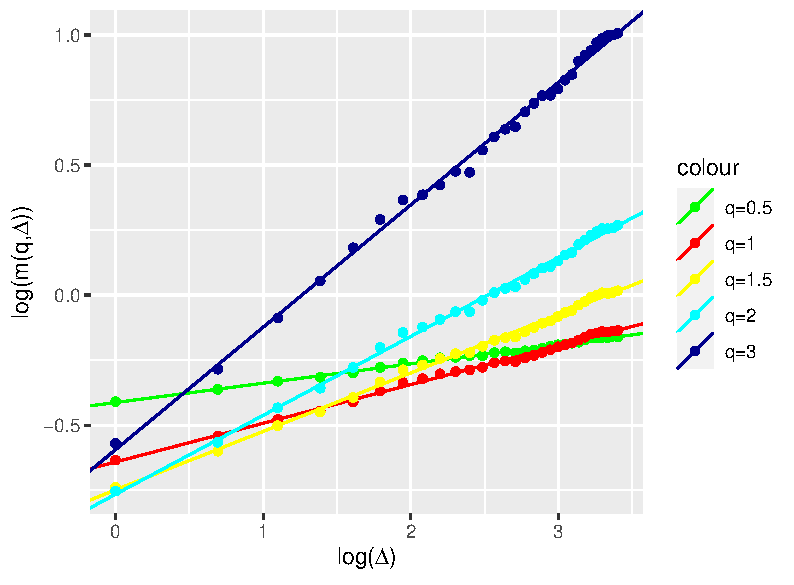
\includegraphics[scale=0.8]{fig/img/RealizedLib/LinearReg.pdf}
    \caption{Caption}
    \label{fig:enter-label}
\end{figure}
%For our rough stochastic volatility model, the underlying asset $S_{t}$ follows the SDE
%\begin{equation}
%    dS_{t}=\mu_{t}S_{t}dt + \sigma_{t}S_{t}dB_{t},
%\end{equation}
%where $\mu_{t}$ is the drift process, which may be deterministic, and $\sigma_{t}$ is the volatility process. The volatility process satisfies 
%\begin{align}
%    dY_{t}&= -\lambda(Y_{t}-\theta)dt + \varphi dB^{H}_{t}\\
%    \sigma_{t} &= e^{Y_{t}},
%\end{align}
%where $\theta\in \R$ and $\lambda,\varphi >0$.